\chapter{Podržano učenje}

Strojno učenje \engl{Machine Learning} jest grana umjetne inteligencije \engl{Artificial Inteligence} koja se može definirati kao skup metoda koje u podatcima mogu automatski otkrivati obrasce, i potom te otkrivene obrasce iskorištavati pri budućem predviđanju podataka, ili obavljati druge zadatke odlučivanja u prisustvu nesigurnosti \cite{CupicUvod}. Drugim riječima, bez eksplicitnog programiranja moguće je napraviti sustave koji funkcioniraju kao ljudski mozak - imaju pristup podatcima, koriste ih za učenje i samim time bolje razumiju entitete, domene i veze između podataka. 

Strojno učenje dijeli se na 3 podvrste: nadzirano učenje, nenadzirano učenje i podržano (ojačano) učenje. Nadzirano učenje \engl{supervised learning} karakterizira učenje modela nad testnim podatcima koji su označeni. Model točno zna da za određeni ulaz mora vratiti izlaz koji je istovjetan unaprijed pridruženoj oznaci. Algoritam mjeri točnost kroz funkciju gubitka, prilagođavajući se sve dok se izračunata razlika izlaza modela i stvarnog izlaza (pogreška) ne smanji u određenoj mjeri. U nenadziranom učenju \engl{unsupervised learning} za razliku od nadziranog, posjedujemo podatke bez zadanog izlaza - podatci su dani bez ciljne vrijednosti i u tim situacijama treba pronaći određenu pravilnost. Postupci poput grupiranja, smanjenja dimenzionalnosti, otkrivanja veza između primjeraka... pripadaju nenadziranom učenju.

Posebna i nama najzanimljivija podvrsta strojnog učenja jest podržano učenje \engl{reinforcement learning}. Podržano učenje bavi se optimizacijom ponašanja agenta koji je u interakciji s okolinom (u kojoj se nalazi) i koji na temelju informacija koje dobiva iz okoline izvršava akcije, i kao odgovor na svaku akciju dobiva nagradu ili kaznu. Za razliku od prethodno dvije navedene podvrste koje mapiraju ulazne podatke na određeni format izlaza, u podržanom učenju je naizraženije učenje iz iskustva koje je čovjeku kao biću ključan način na koji se razvija. Od najranije dobi, bića nastoje shvatiti i razumjeti okolinu u kojoj se nalaze na temelju niza aktivnosti kojima utječu na okolinu i opažanja kako okolina pri toj interakciji utječe na nas. 

\section{Ključni koncepti}

% https://spinningup.openai.com/en/latest/spinningup/rl_intro.html 

Za potpuno razumijevanje podržanog učenja, bitno je u navesti i pojasniti glavne pojmove. Okolina \engl{environment} označava svijet u kojem se agent nalazi i s kojim interaktira. Stanje \engl{state} reprezentira presjek okoline u određenom trenutku. Agentu korisna informacija jest nagrada \engl{reward} koja predstavlja povratnu informaciju okoline. Način na koji agent bira akciju \engl{action} iz skupa svih dostupnih akcija naziva se politika \engl{policy}.



Cilj podržanog učenja jest naći optimalnu strategiju (niz optimalnih akcija) koje maksimiziraju ukupnu (kumulativnu) nagradu. U svakom koraku interakcije agenta s okolinom, agent prima opis stanja okoline u kojoj se nalazi. S obzirom na to stanje, izvršava akciju koja vrši neku promjenu nad okolinom i prebacuje ju u novo stanje. Agent prima povratnu informaciju od okoline koja reprezentira koliko je odabrana akcija u skladu sa stanjem okoline. Opisana interakcija agenta s okolinom prikazana je na slici \ref{fig:rl}.

\begin{figure}[h]
    \centering
    \frame{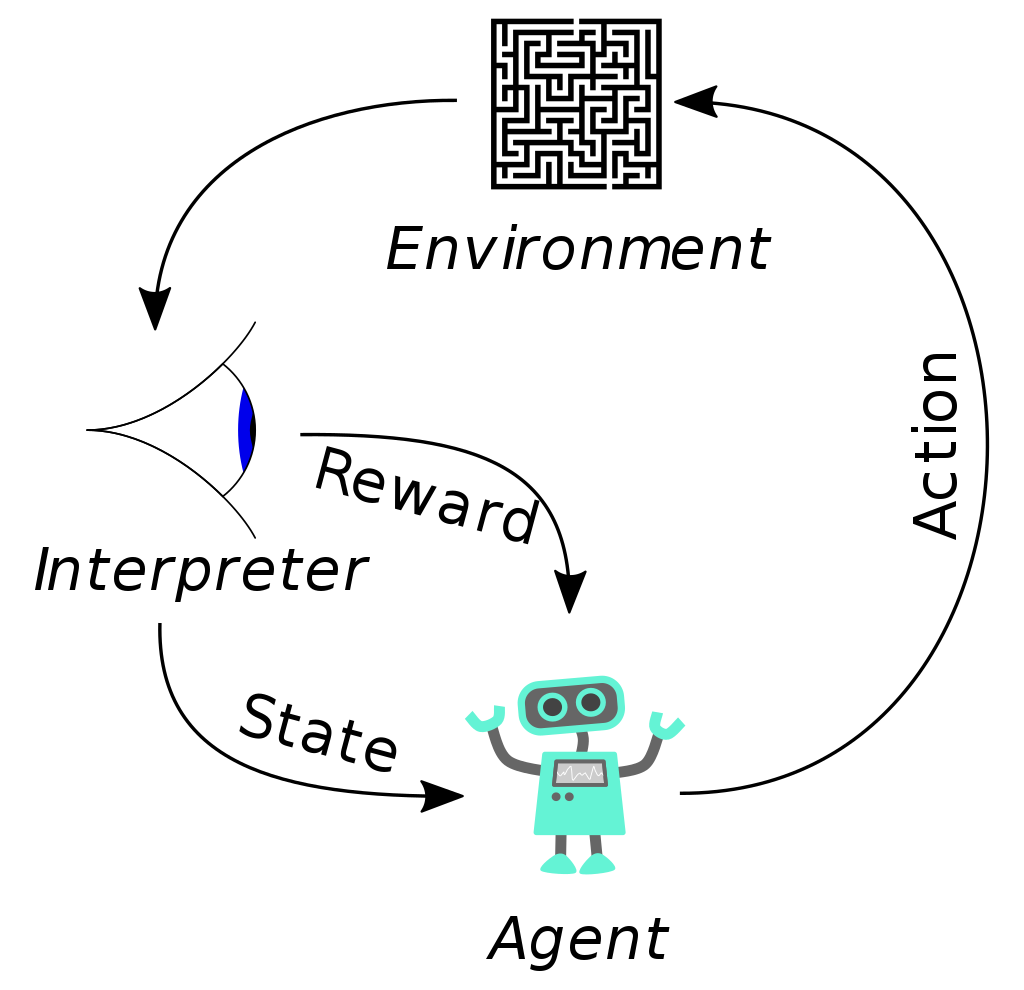
\includegraphics[width=7cm]{assets/rl_diagram.png}}
    \caption{Prikaz ciklusa i interakcije agenta s okolinom}
    \label{fig:rl}
\end{figure}

\section{Duboki modeli}

Duboko učenje \engl{Deep learning} jest tip strojnog učenja (točnije, podskup strojnog učenja) koje nastoji oponašati način zaključivanja i obrasce koje ljudski mozak koristi za učenje i donošenje odluka. Veliku ulogu u cijeloj ideji dubokog učenja imaju duboke neuronske mreže \engl{Deep neural networks, DNN} pomoću kojih se povezivanjem više slojeva procesnih elemenata (čvorova, neurona), dobivaju duboki modeli koji su sposobni učiti i baratati s podatcima kompozitne strukture. Primjenom dubokih modela dolazimo do slijeda naučenih nelinearnih transformacija kojima aproksimiramo funkciju odluke, učimo mapiranje između ulaznih podataka i izlazih podataka, te nastojimo postići dobru generalizaciju nad stvarnim podatcima. 

\subsection{Unaprijedni potpuno povezani modeli}

Unaprijedni potpuno povezani modeli \engl{Fully connected neural network} (poznatiji i pod nazivom višeslojni perceptron \engl{Multi-layer perceptron}) sastoje se od lanaca potpuno povezanih slojeva. Svaki neuron iz prethodnog sloja povezan je s neuronom idućeg sloja. 

Sastoje se od tri vrste slojeva - ulaznog sloja, izlaznog sloja i skrivenih slojeva. Ulaznom sloju dovode se podatci koje je potrebno obraditi. Izlaz neuronske mreže (u najosnovnijem obliku) predstavljen je logitima \engl{logits} - vektorima logaritama nenormaliziranih vrijednosti. Specifičnije, za slučaj da želimo provesti klasifikaciju podataka ili drugačije organizirati izlazne vrijednosti na izlaz dodajemo posebni sloj (npr. \textit{Softmax} funkcija za klasifikaciju). Samo su ulaz i izlaz specificirani dimenzijama. Model ima slobodu da iskoristi skrivene slojeve na način koji osigurava najbolju aproksimaciju funkcije. Neuronskim mrežama želimo izgraditi modele koji nisu linearno odvojivi i zato koristimo nelinearnu aktivacijsku funkciju - najčešće ReLU (Rectified Linear Unit). Svaki od slojeva modelira jednu nelinearnu transformaciju.

Slika \ref{fig:nn} prikazuje arhitekturu potpuno povezanog modela \cite{NNsvg} koji je sastavljen od sveukupno 4 potpuno povezana sloja - ulaznog (dimenzije 4), izlaznog (dimenzije 2) i dva skrivena sloja (svaki dimenzije 8). Kodom \ref{lst:fcn} prikazana je implementacija navedenog modela u biblioteci \textit{PyTorch}.

\begin{figure}[H]
    \centering
    \frame{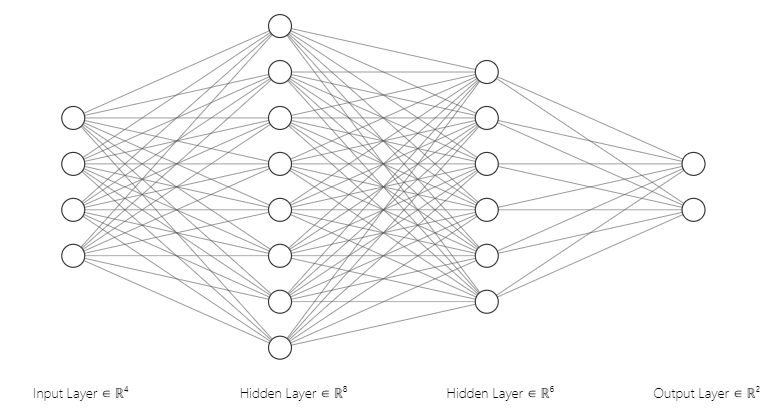
\includegraphics[width=9cm]{assets/nn.png}}
    \caption{Prikaz arhitekture potpuno povezanog modela}
    \label{fig:nn}
\end{figure}

\begin{listing}[H]
    \caption{Implementacija potpuno povezanog modela na slici \ref{fig:nn} koristeći biblioteku \textit{PyTorch}}
    \inputminted{python}{snippets/fcn.py}
    \label{lst:fcn}
\end{listing}

\subsection{Konvolucijski modeli}

Konvolucijski modeli \engl{Convolutional neural networks} su modeli koji uz potpuno povezane slojeve imaju najmanje jedan konvolucijski sloj \engl{Convolution layer}. Osim spomenutog konvolucijskog sloja i potpuno povezanog sloja, konvolucijski modeli sadrže i slojeve sažimanja \engl{Pooling layers}, slojeve u kojima provodimo nelinearnost te sloj koji višedimenzionalni ulaz pretvara u jednodimenzionalni i pritom priprema podatke za obradu u potpuno povezanim slojevima \engl{Flatten layer}.

Operacija konvolucije provodi se nad ulazom i jezgrom \engl{kernel} (slobodnim parametrima koje učimo) gdje kao rezultat dobivamo mapu značajki koja pokazuje gdje se koja značajka nalazi u ulaznim podatcima (npr. slici). Dimenzije mapa značajki i njihovu robusnost korigiramo korištenjem atributa koraka konvolucije \engl{stride} i nadopunjavanja ulaznih podataka \engl{padding}. Slično konvolucijskom sloju, sloj sažimanja odgovoran je za smanjenje prostora značajki (smanjenje dimenzionalnosti podataka) i dodatno za izdvajanje dominantnih značajki. Razlikujemo dvije vrste sažimanja: sažimanje maksimalnom vrijednosti \engl{Max pooling} i sažimanje srednjom vrijednosti \engl{Average pooling}. Prilikom sažimanja značajki maksimalnom vrijednošću u obzir uzimamo samo značajku najveće vrijednosti (potencijalno najvažniju značajku) te na taj način uklanjamo šum ulaza.

Korištenje konvolucijskih modela biti će nam iznimno potrebno u situacijama kada su ulazni podatci u formi slike, odnosno kada su nam važne lokalne interakcije između ulaznih podataka (piksela) te njihova vremenska i prostorna ovisnost.

Slika \ref{fig:cnn} prikazuje jednostavni konvolucijski model koji se sastoji od konvolucijskog sloja, sloja sažimanja maksimalnom vrijednosti, sloja koji 3-dimenzionalne podatke pretvara u 1-dimenzionalne, te dva potpuno povezana sloja. Ulaz u konvolucijski sloj predstavlja RGB slika (3 kanala) dimenzije $32 \times 32$. Primjenom konvolucije (veličina jezgre 3, korak 3, nadopuna 1) izvlačimo 18 kanala značajki dimenzije $32 \times 32$ (dimenzija se nije promijenila iz razloga što nadopunjavamo ulaz). Primjenom sažimanja maksimumom (veličina jezgre 2, korak 2) smanjujemo broj značajki na dimenziju $16 \times 16$. Prvi potpuno povezani sloj na svoj ulaz dobije vektor dimenzije $4608$ kojeg pretvara u vektor izlaza dimenzije $64$. Posljednji potpuno povezani sloj koji je ujedno i posljednji sloj u ovom konvolucijskom modelu za izlaz predaje vektor dimenzije $10$. Isječak koda koji prikazuje implementaciju jednostavnog konvolucijskog modela koristeći bibilioteku \textit{PyTorch} prikazan je kodom \ref{lst:cnn}.

\begin{figure}[H]
    \centering
    \frame{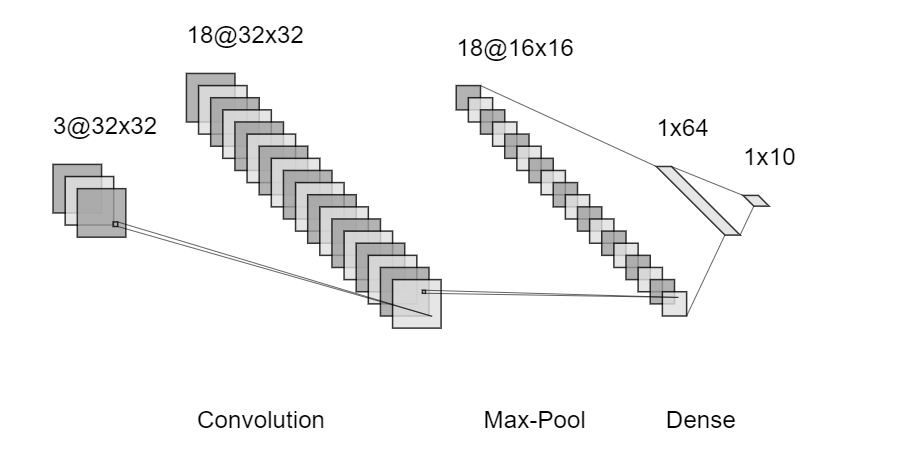
\includegraphics[width=11cm]{assets/cnn.png}}
    \caption{Prikaz arhitekture konvolucijskog modela}
    \label{fig:cnn}
\end{figure}

\begin{listing}[H]
    \caption{Implementacija konvolucijskog modela na slici \ref{fig:cnn} koristeći biblioteku \textit{PyTorch}}
    \inputminted{python}{snippets/cnn.py}
    \label{lst:cnn}
\end{listing}

\section{Algoritmi podržanog učenja}

Onaj dio s towards science oko explorationa...

Svaki model strojnog učenja definiran modelom, gubitkom i metodom optimizacije. Model jest postupak obrade (odnosno skup funkcija) sa slobodnim parametrima koji za određen ulaz daje pripadajući izlaz. Gubitak jest mjera koja na formaliziran način vrednuje slobodne parametre modela, odnosno pokazuje u kojoj mjeri se mi ne slažemo s onim što je model predstavio kao izlaz. Metoda optimizacije (optimizacijski postupak) jest način na koji pronalazimo optimalne parametre koji su važno kako bi minimizirali prethodno navedenu komponentu - gubitak. Navedene tri glavne komponente biti će važno napomenuti pri svakom predstavljaju algoritma jer su to glavne odrednice pri analizi algoritama strojnog učenja.

% dodati literaturu https://www.fer.unizg.hr/_download/repository/SU-2020-02-OsnovniKoncepti.pdf

\subsection{Deep Q Learning}
\subsection{Double Deep Q Learning}
\subsection{Actor Critic}

% faza učenja modela, faza iskorištavanja modela